\documentclass{scrartcl}

\usepackage[utf8]{inputenc}
\usepackage[T1]{fontenc}
\usepackage[ngerman]{babel}
\usepackage{amssymb}
\usepackage{amsmath}
\usepackage{mathtools}
\usepackage{graphicx}
\usepackage{framed}
\usepackage{xcolor}
\usepackage[nottoc]{tocbibind}
\usepackage{caption}

\colorlet{shadecolor}{gray!25}
\setlength{\parindent}{0pt}

\newcommand{\abs}[1]{\left\lvert#1\right\rvert}


\begin{document}

\title{Lösen des Poisson-Problems mittels Finite-Differenzen-Diskretisierung\\
und CG-Verfahren}
\author{Marisa Breßler und Anne Jeschke (PPI27)}
\date{07.02.2020}
\maketitle

\tableofcontents

\pagebreak
\section{Motivation}
In unserem vorherigen Berichten haben wir das Poisson-Problem vorgestellt und einen numerischen Lösungsansatz aufgezeigt, der es durch eine Diskretisierung des Gebietes und des Laplace-Operators in das Lösen eines linearen Gleichungssystems überführt.
Die dabei entstehende tridiagonale Blockmatrix ist dünn besetzt, d.h. nur wenige Einträge sind ungleich Null.
Deswegen ist es sinnvoll, sie als sogenannte \textit{sparse}-Matrix abzuspeichern.
Dieser Speicherplatzvorteil geht jedoch beim Lösen des linearen Gleichungssystems mittels Gauß-Algorithmus und LU-Zerlegung verloren, da eine LU-Zerlegung einer dünn besetzten Matrix im Allgemeinen nicht dünn besetzt ist.
Aufgrund dieses Umstandes erscheint es sinnvoll, das lineare Gleichungssystem nicht direkt, sondern iterativ zu lösen.
Solche iterativen Lösungsverfahren (wie das Gesamtschrittverfahren von Jacobi, das Einzelschrittverfahren von Gauß-Seidel, das SOR-Verfahren und das CG-Verfahren) bieten gegenüber direkten Verfahren außerdem den Vorteil, dass deren Rechenaufwand im Verhältnis zur in der Praxis für gewöhnlich sehr großen Dimension der Blockmatrix recht gering ist.
Da das CG-Verfahrens eine heute durchaus übliche Methode zum Lösen großer linearer Gleichungssysteme darstellt, wollen wir dieses im Folgenden im Rahmen unseres bisherigen Settings (Poisson-Problem und Finite-Differenzen-Diskretisierung) vorstellen und untersuchen.



\pagebreak
\section{Theoretische Grundlagen und Algorithmus}

Im Gegensatz zu den bisher behandelten direkten Verfahren, die nach einer endlichen Anzahl von Rechenschritten den Lösungsvektor $x$ des linearen Gleichungssystems $Ax=b$ mit $A\in\mathbb{R}^{N\times N}$ und $b\in\mathbb{R}^N$ liefern, definiert man bei den iterativen Verfahren eine Folge $(x_k)$ von Vektoren, die bei einem beliebigen Vektor startet und deren Grenzwert für $k \to \infty$ der genaue Lösungsvektor ist.
Man wählt dann ein $\epsilon\in\mathbb{R}$ und berechnet so viele Iterationsschritte, bis das Residuum, also der approximierte Abstand des in diesem Schritt berecheten Folgenelementes zu der exakten Lösung, kleiner als $\epsilon$ ist.

Das CG-Verfahren (kurz für \textit{conjugated gradient}) ist ein Verfahren, das nur für symmetrisch positiv definite Matrizen $A$ funktioniert.
Diese Voraussetzung wird von unserer Blockmatrix erfüllt, denn sie ist per Definition symmetrisch und irreduzibel diagonaldominant.

\subsection{Idee des CG-Verfahrens}

Während sich die anderen oben genannten iterativen Verfahren die Methode des Splitting zunutze machen, ist die Idee des CG-Verfahrens die Lösung des linearen Gleichungssystems in ein Minimierungsproblem zu überführen.

Dazu definiert man mit dem Standardskalarprodukt $<.,.>$ die Funktion
\begin{align*}
  \Phi (x) &\coloneqq \frac{1}{2}<x,Ax> - <b,x>\\
           &=\frac{1}{2}x^T Ax - x^T b
\end{align*}

Diese besitzt genau ein globales Minimum. Dieses liegt genau an der Stelle $x$, die der Lösung von $Ax=b$ entspricht. Man konstruiert also, um die Lösung von $Ax=b$zu finden, iterativ eine Folge von immer kleiner werdenden Funktionswerten von $\Phi$.\\

Um das globale Minimum zu finden, sucht man ausgehend von einem Startwert zunächst nach dem Minimum entlang einer Startrichtung (eines Startgradienten).
Von diesem Minimum aus wählt man eine neue Suchrichtung (einen neuen Gradienten), die zu allen vorherigen Suchrichtungen $A$-konjugiert, d.h. orthogonal in der $A$-Norm, ist und sucht erneut nach einem Minimum entlang dieses Gradienten.
Dies tut man so lange, bis das Residuum kleiner oder gleich $\epsilon$ ist.
Da es nur genau $N$ zueinander $A$-konjugierte Richtungen gibt, würde man mit dem CG-Verfahren in der Theorie nach maximal $N$ Schritten sogar die exakte Lösung finden.
In der Praxis benötigt man jedoch den Toleranzfaktor $\epsilon$, da durch Rundungsfehler die Suchrichtungen unter Umständen nicht mehr genau orthogonal zueinander stehen und diese Garantie somit verloren geht.\\

\subsection{Algorithmus}

\underline{Initialisierung}: Man startet bei einem beliebigen $x_0\in\mathbb{R}^N$ und wählt einen Toleranzfaktor $\epsilon$.
Man setzt $k\coloneqq 0$ und berechnet das Anfangsresiduum $r_0 \coloneqq Ax_0 - b$. Die erste Suchrichtung ist $d_0 = -r_0$.\\

\underline{Schritt k}: Falls $||r_k||\leq \epsilon$, hat man bereits eine Lösung im Toleranzbereich gefunden und kann hier aufhören.

Sonst berechnet man $c_k \coloneqq <r_k, r_k>/<Ad_k,d_k>$. Dies gibt an, wie weit man in die Suchrichtung gehen muss, um das neue Minimum zu finden.

Dann gilt $x_{k+1} = x_k + c_k d_k$ und $r_{k+1} = r_k + c_k Ad_k = Ax_{k+1} - b$.

Man setzt $\beta_k \coloneqq <g_{k+1},g_{k+1}>/<g_{k},g_{k}>$.

Die neue zu $d_k$ $A$-konjugierte Suchrichtung ist dann $d_{k+1}\coloneqq -r_{k+1} + \beta_k d_k$.

Nun setzt man $k \coloneqq k+1$ und geht erneut zu Schritt k.\\

So nähert man sich Schritt für Schritt einer genauen Lösung von $Ax=b$.
Um zu verhindern, dass der Algorithmus für sehr viele Iterationen läuft ohne, dass sich das Ergebnis signifikant verbessert, kann man zusätzliche Abbruchbedingungen definieren, wie z.B. eine minimale Reduktion des Residuums nach jedem Schritt oder eine maximale Anzahl der Iterationsschritte.

\cite{tischendorf2019}

\pagebreak
\section{Experimente und Beobachtungen}
Im Folgenden wollen wir verschiedene Experimente präsentieren. 
Da wir im Gegensatz zu unserer Arbeit vom 03.01.2020 in hiesigen Rahmen das Gleichungssystem nicht direkt mittels Gauß-Algorithmus und LU-Zerlegung, sondern iterativ mittels CG-Verfahren lösen, gilt unser Interesse der Vorstellung der neuen Methode zum Ermitteln einer Lösung des Poisson-Problems sowie der Gegenüberstellung der beiden Verfahrensweisen.  


\subsection{Entwicklung des absoluten Fehlers pro Iteration}
Während direkte Verfahren nach einer endlichen Anzahl an Rechenoperationen \glqq{die exakte Lösung}\grqq{} liefern (dabei handelt es sich in Praxis nicht um die exakte analytische Lösung, da ein Computer aufgrund seiner begrenzten Rechenleistung im Allgemeinen immer bei der Verarbeitung von Zahlen Fehler produziert), ermitteln iterative Verfahren schrittweise eine immer bessere Approximation der gesuchten Lösung. \\ 
Diese sukzessive Annäherung an die exakte Lösung lässt sich an den folgenden drei Grafiken erkennen. 
Diese zeigen jeweils für den ein-, den zwei- und den dreidimensionalen Fall die Entwicklung des absoluten Fehlers pro Iteration. 
Der Graph schmiegt sich immer mehr der y-Achse an. 
Dieses asymptotische Fehlerverhalten ist charakteristisch für iterative Verfahren. \\

{
  \centering
    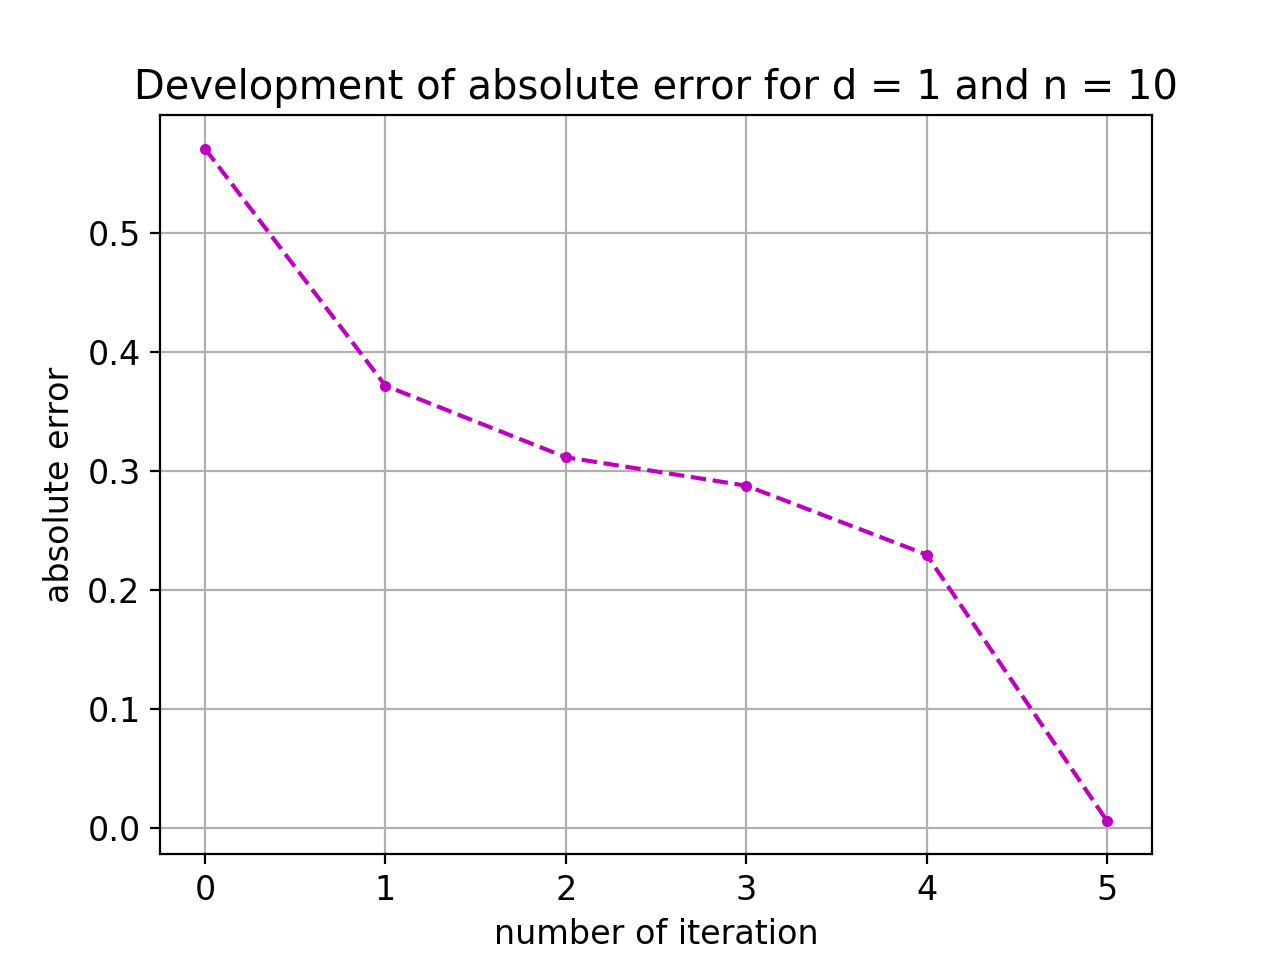
\includegraphics[width=0.45\textwidth]{Grafiken/iterates_d1_n10}
    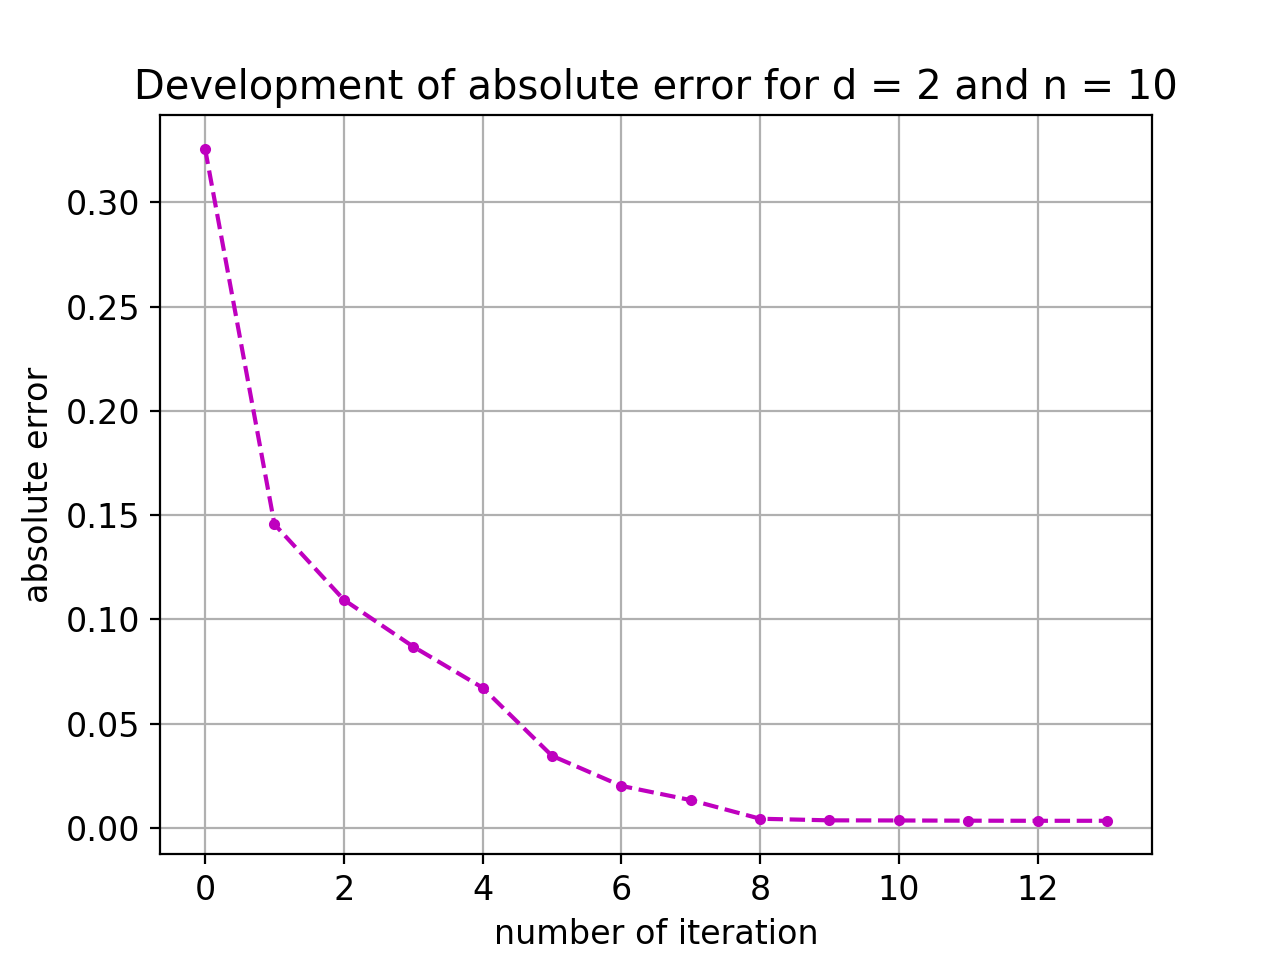
\includegraphics[width=0.45\textwidth]{Grafiken/iterates_d2_n10}
    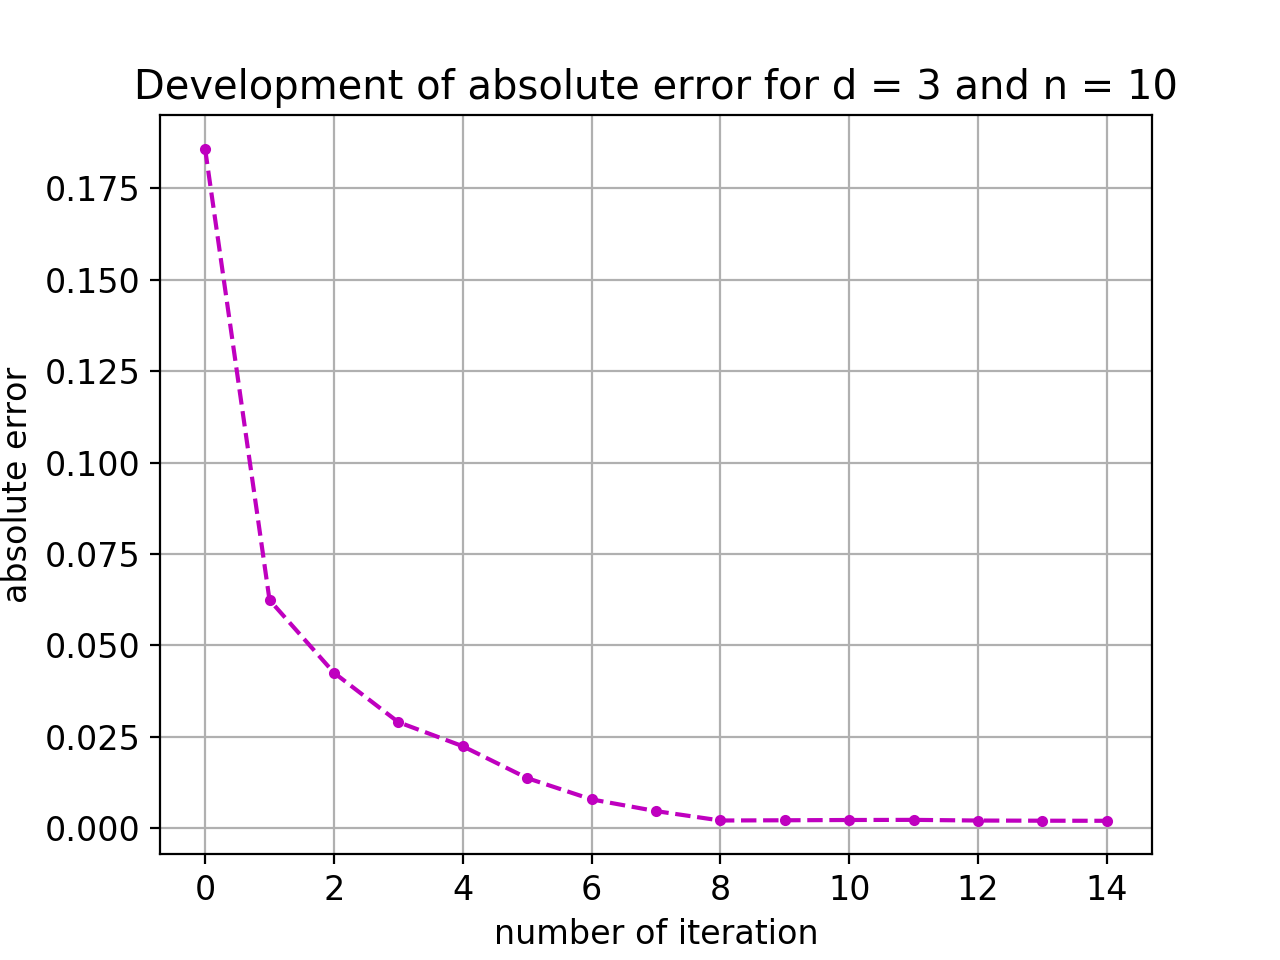
\includegraphics[width=0.45\textwidth]{Grafiken/iterates_d3_n10}
    \vspace{-0.2cm}
    \captionof{figure}{Entwicklung des absoluten Fehlers pro Iteration für $d\in\{1, 2, 3\}$ und $n=10$}
}
\vspace{0.5cm}

Darüber hinaus ist auffallend, dass weitaus weniger als $N=(n-1)^d$ Schritte vonnöten sind, um eine sehr gute Näherungslösung zu errechnen. 
Während wir im eindimensionalen Fall, $N=9$, bereits nach der fünften Iteration eine ausreichend genaue Lösung haben, benötigen wir im zweidimensionalen Fall, $N=81$, nur 13 und im dreidimensionalen Fall, $N=729$ lediglich eine mehr, nämlich 14 Iterationen.  
(Die große Konvergenzgeschwindigkeit lässt sich auf die gute Kondition der tridiagonalen Blockmatrix zurückführen.) 
Doch bei allen ist der Fehler schon nach acht Schritten nur noch sehr gering. 
Dass unser Programm dennoch weiterrechnet, ist den Umstand geschuldet, dass noch keiner der eingegebenen Abbruchparameter zum Tragen kam. 
Da die Rechenschritte bei direkten Verfahren wie gesagt im Voraus bekannt und begrenzt sind, bei iterativen jedoch nicht, benötigen letztere Abbruchbedingungen, die den Schleifendurchlauf des Algorithmus zum Ende bringen. 
Unsere Implementierung der Methode der konjugierten Gradienten (CG) enthält die folgenden drei Abbruchbedingungen. 
\glqq{eps}\grqq: Abbruch, falls die Norm des Residuums eine vorgegebene Grenze unterschreitet, \glqq{max\_iter}\grqq: Abbruch, falls eine vorgegebene Anzahl an Iterationen erreicht ist, \glqq{min\_red}\grqq: Abbruch, falls das Verfahren \glqq{feststeckt}\grqq, d.h. falls der Abstand zwischen den letzten beiden Residuen eine vorgegebene Grenze unterschreitet. ... \\

\pagebreak
\subsection{Konvergenzverhalten für ein festes Epsilon}
gleiches Konvergenzverhalten wie LU \\
Konvergenz abh. von Diskretisierung, nicht von Lösungsverfahren\\

{
  \centering
    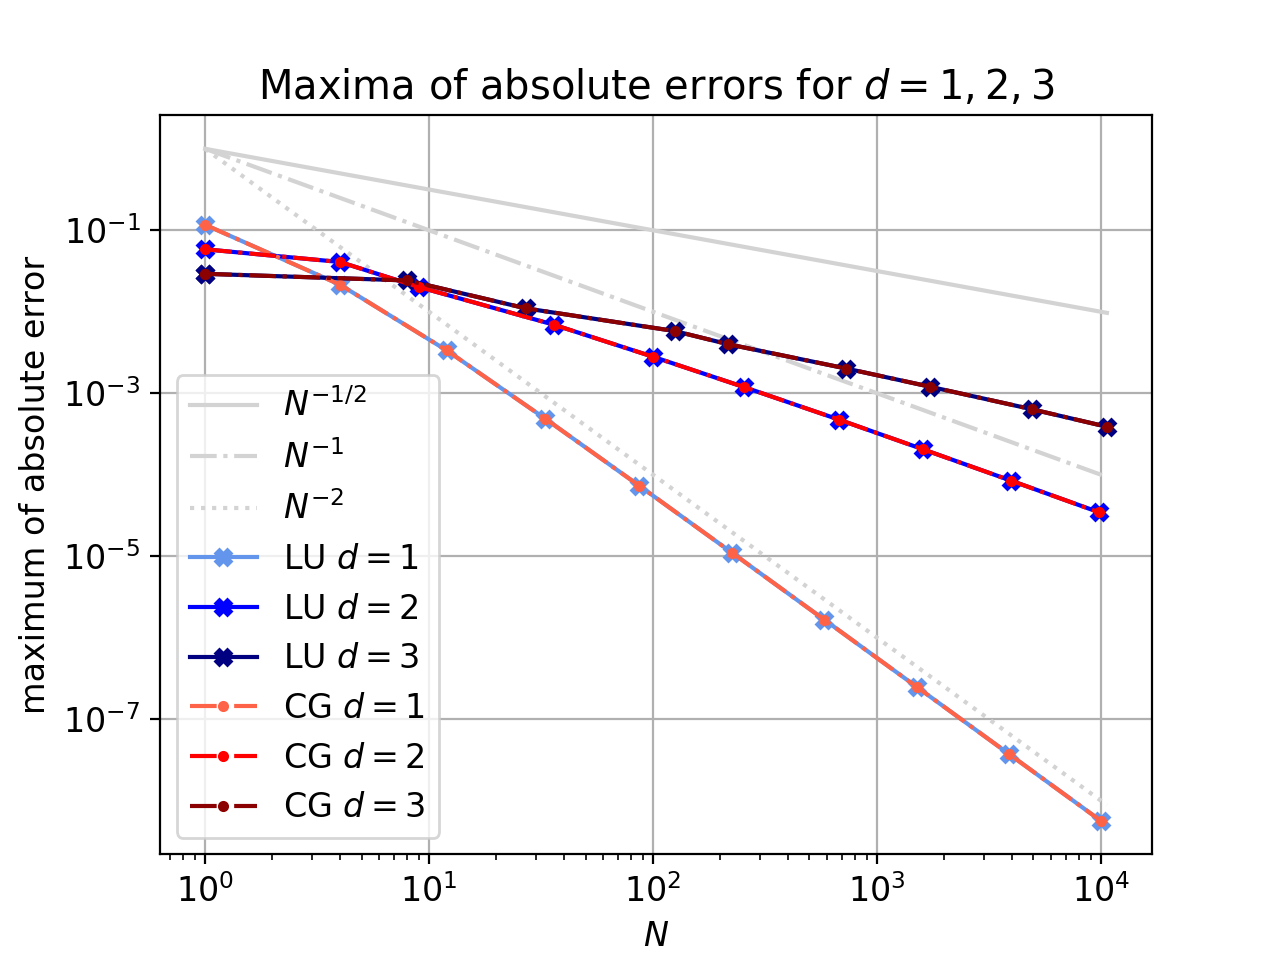
\includegraphics[width=0.75\textwidth]{Grafiken/compare}
    \vspace{-0.2cm}
    \captionof{figure}{Vergleich Konvergenzverhalten LU und CG mit $\epsilon = 10^{-8}$ für $d\in\{1, 2, 3\}$}
}
\vspace{0.5cm}


\pagebreak
\subsection{Konvergenzverhalten für variable Epsilon}


{
  \centering
    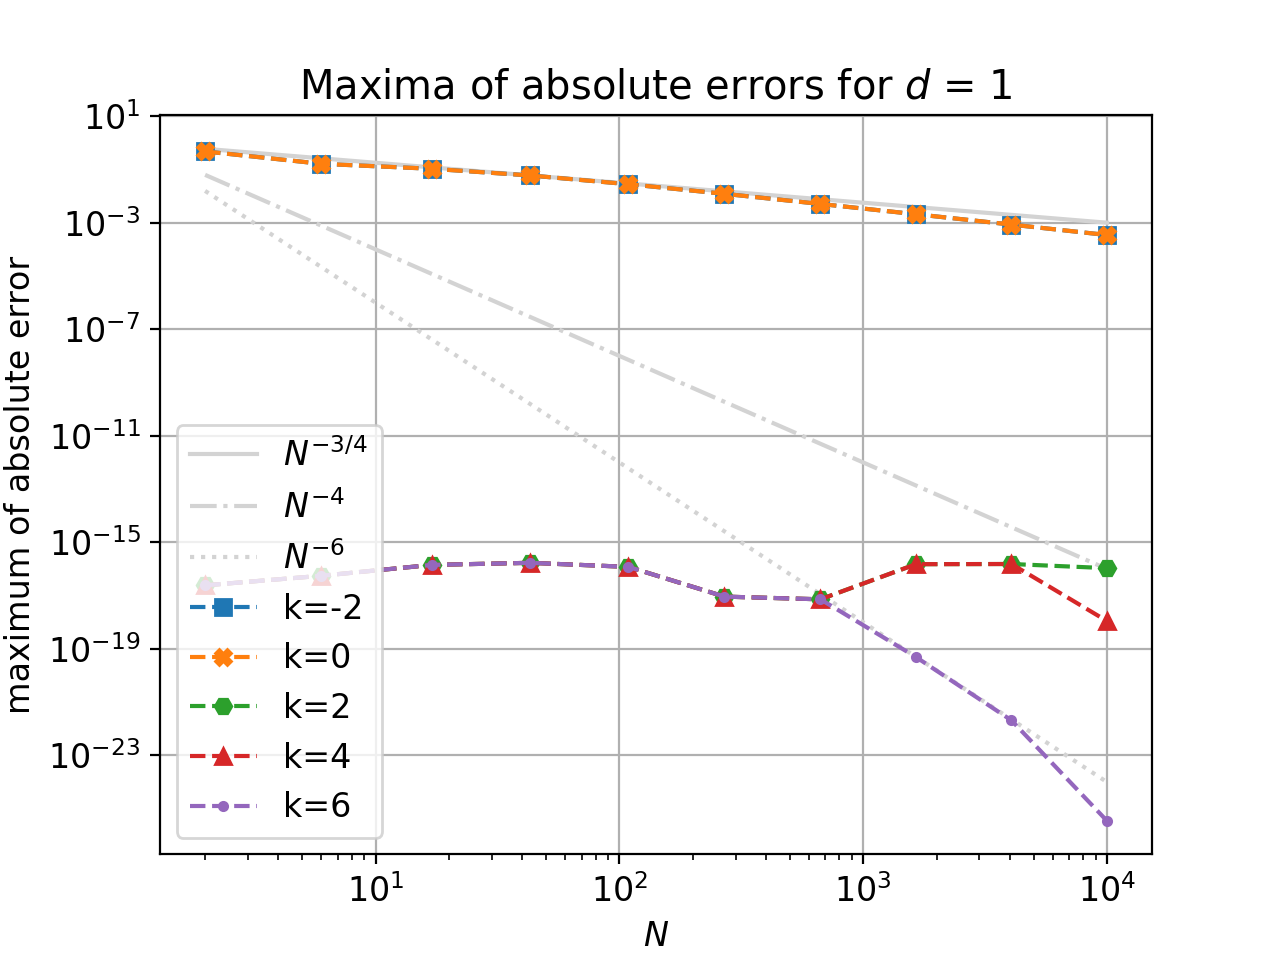
\includegraphics[width=0.45\textwidth]{Grafiken/epsilon_d1}
    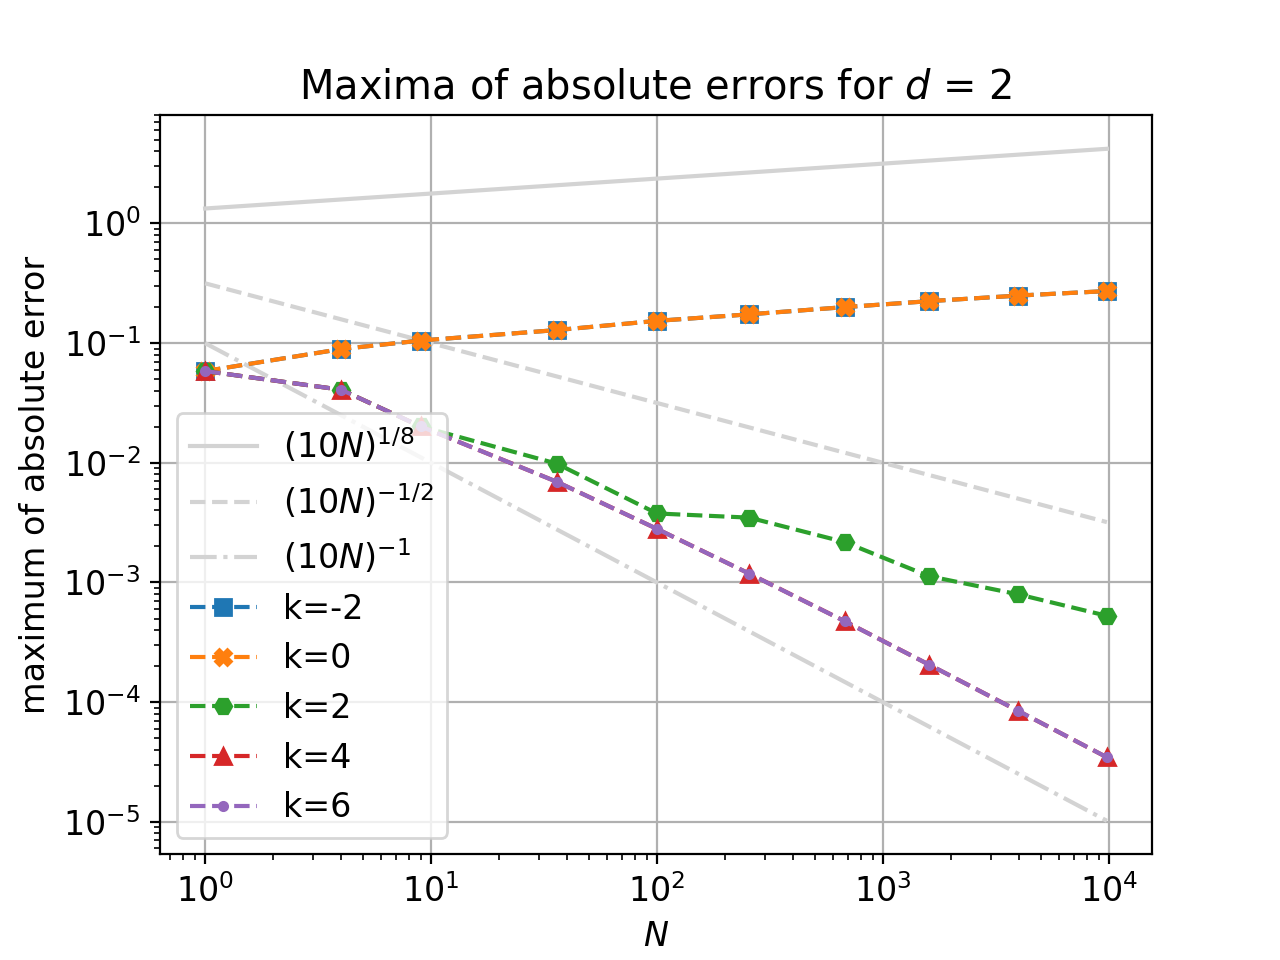
\includegraphics[width=0.45\textwidth]{Grafiken/epsilon_d2}
    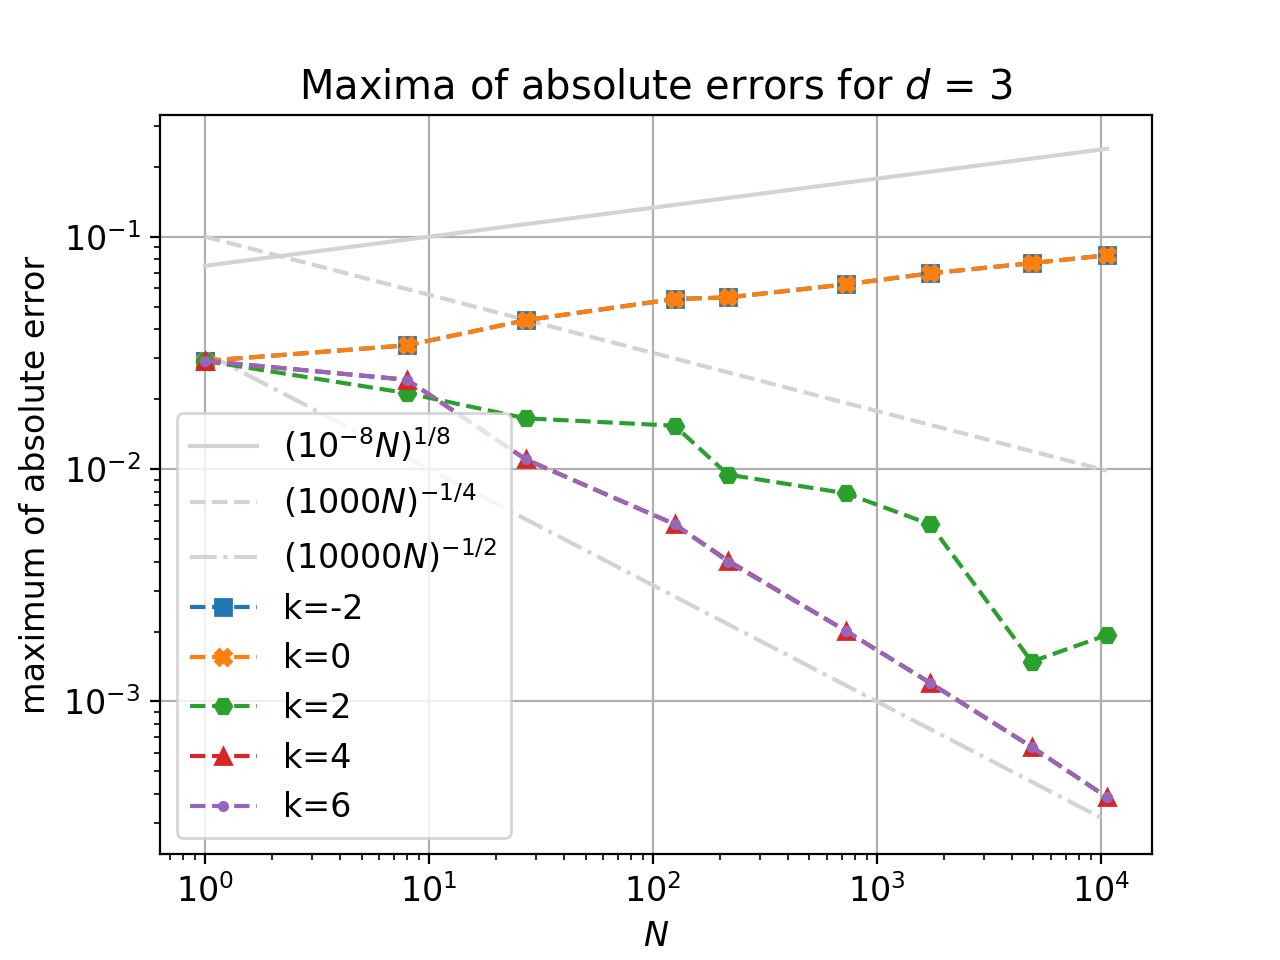
\includegraphics[width=0.45\textwidth]{Grafiken/epsilon_d3}
    \vspace{-0.2cm}
    \captionof{figure}{Konvergenzverhalten mit $\epsilon^{(k)}=n^{-k}$ für $d\in\{1, 2, 3\}$}
}
\vspace{0.5cm}


\pagebreak
\section{Abschließende Worte}

\pagebreak
\bibliographystyle{plain}
\bibliography{serie5_literatur}

\end{document}
